\documentclass{article}

\usepackage{amsmath}
\usepackage{graphicx}

\newcommand{\andSp}{\ \mathrm{and}\ }

\begin{document}
\title{APMA 4301: Problem Set 2}
\author{Brian Dawes}
\date{\today}
\maketitle
\section*{Problem 1}
\subsection*{a)}
Using the Taylor expansion, we can write:
\begin{equation}
u(x) = u(\bar x)+(x-\bar x)u'(\bar x)+\frac{(x-\bar x)^2}{2}u''(\bar x)+\frac{(x-\bar x)^3}{6}u^{(3)}(\bar x)
\end{equation}

Plugging in $x=0,h,2h$, we get:
\begin{eqnarray}
u_0 \approx u(\bar x)-\bar xu'(\bar x)+\frac{\bar x^2}{2}u''(\bar x)-\frac{\bar x^3}{6}u^{(3)}(\bar x) \\
u_1 \approx u(\bar x)+(h-\bar x)u'(\bar x)+\frac{(h-\bar x)^2}{2}u''(\bar x)+\frac{(h-\bar x)^3}{6}u^{(3)}(\bar x) \\
u_2 \approx u(\bar x)+(2h-\bar x)u'(\bar x)+\frac{(2h-\bar x)^2}{2}u''(\bar x)+\frac{(2h-\bar x)^3}{6}u^{(3)}(\bar x)
\end{eqnarray}
where $u_0=u(0)$, $u_1=u(h)$, and $u_2=u(2h)$.

Now we want to find stencil weights $s_0,s_1,s_2$ and $s_0',s_1',s_2'$ such that:
\begin{gather}
s_0u_0+s_1u_1+s_2u_2=u'(\bar x) \\
s_0'u_0+s_1'u_1+s_2'u_2=u''(\bar x)
\end{gather}

This can be represented in matrix form as:
\begin{equation}
\begin{bmatrix}
1 & 1 & 1 \\
-\bar x & h-\bar x & 2h-\bar x \\
\bar x^2/2 & (h-\bar x)^2/2 & (2h-\bar x)^2/2
\end{bmatrix}
\begin{bmatrix}
s_0 \\ s_1 \\ s_2
\end{bmatrix}
=
\begin{bmatrix}
0 \\ 1 \\ 0
\end{bmatrix}
\ \mathrm{or}\ 
\begin{bmatrix}
0 \\ 0 \\ 1
\end{bmatrix}
\end{equation}
which can be solved from the matrix:
\begin{equation}
\begin{bmatrix}
1 & 1 & 1 & 0 & 0\\
-\bar x & h-\bar x & 2h-\bar x & 1 & 0\\
\bar x^2/2 & (h-\bar x)^2/2 & (2h-\bar x)^2/2 & 0 & 1
\end{bmatrix}
\end{equation}

\subsubsection*{Case 1: $\bar x=0$}
Our matrix becomes:
\begin{align*}
\begin{bmatrix}
1 & 1 & 1 & 0 & 0\\
0 & h & 2h & 1 & 0\\
0 & h^2/2 & 2h^2 & 0 & 1
\end{bmatrix}
&\to
\begin{bmatrix}
1 & 1 & 1 & 0 & 0\\
0 & h & 2h & 1 & 0\\
0 & 0 & h^2 & -h/2 & 1
\end{bmatrix} \\
&\to s_2=-1/2h\andSp s_2'=1/h^2 \\
&\to s_1=2/h\andSp s_1'=-2/h^2 \\
&\to s_0=-3/2h\andSp s_0'=1/h^2
\end{align*}
\begin{equation}
\boxed{(s_0,s_1,s_2)=\frac{1}{2h}(-3,4,-1)\andSp(s_0',s_1',s_2')=\frac{1}{h^2}(1,-2,1)}
\end{equation}

\subsubsection*{Case 2: $\bar x=h/2$}
Our matrix becomes:
\begin{align*}
\begin{bmatrix}
1 & 1 & 1 & 0 & 0\\
-h/2 & h/2 & 3h/2 & 1 & 0\\
h^2/8 & h^2/8 & 9h^2/8 & 0 & 1
\end{bmatrix}
&\to\begin{bmatrix}
1 & 1 & 1 & 0 & 0\\
0 & h & 2h & 1 & 0\\
0 & 0 & h^2 & 0 & 1
\end{bmatrix} \\
&\to s_2=0\andSp s_2'=1/h^2 \\
&\to s_1=1/h\andSp s_1'=-2/h^2 \\
&\to s_0=-1/h\andSp s_0'=1/h^2
\end{align*}
\begin{equation}
\boxed{(s_0,s_1,s_2)=\frac{1}{h}(-1,1,0)\andSp(s_0',s_1',s_2')=\frac{1}{h^2}(1,-2,1)}
\end{equation}
\subsubsection*{Case 3: $\bar x=h$}
Our matrix becomes:
\begin{align*}
\begin{bmatrix}
1 & 1 & 1 & 0 & 0\\
-h & 0 & h & 1 & 0\\
h^2/2 & 0 & h^2/2 & 0 & 1
\end{bmatrix}
&\to
\begin{bmatrix}
1 & 1 & 1 & 0 & 0\\
-h & 0 & h & 1 & 0\\
0 & 0 & h^2 & h/2 & 1
\end{bmatrix} \\
&\to s_2=1/2h\andSp s_2'=1/h^2 \\
&\to s_0=-1/2h\andSp s_0'=1/h^2 \\
&\to s_1=0\andSp s_1'=-2/h^2
\end{align*}
\begin{equation}
\boxed{(s_0,s_1,s_2)=\frac{1}{2h}(-1,0,1)\andSp(s_0',s_1',s_2')=\frac{1}{h^2}(1,-2,1)}
\end{equation}

\subsection*{b)}
Since we already accounted for the first and second derivatives in the calculation of our stencil weights, our leading error can only come from the third derivative or higher terms in Eqns. 2, 3, and 4.

\subsubsection*{Case 1: $\bar x=0$}
For the first derivative, we get:
\begin{equation}
1/2h(0+2h^3/3-4h^3/3)u^{(3)}(0)=\boxed{-\frac{h^2}{3}u^{(3)}(0)}
\end{equation}
and for the second derivative, we get:
\begin{equation}
1/h^2(0-h^3/3+4h^3/3)u^{(3)}(0)=\boxed{hu^{(3)}(0)}
\end{equation}

\subsubsection*{Case 2: $\bar x=h/2$}
For the first derivative, we get:
\begin{equation}
1/h(h^3/48+h^3/48+0)u^{(3)}(h/2)=\boxed{-\frac{h^2}{24}u^{(3)}(h/2)}
\end{equation}
and for the second derivative, we get:
\begin{equation}
1/h^2(-h^3/48-h^3/24+9h^3/16)u^{(3)}(h/2)=\boxed{\frac{h}{2}u^{(3)}(h/2)}
\end{equation}

\subsubsection*{Case 3: $\bar x=h$}
For the first derivative, we get:
\begin{equation}
1/2h(h^3/6+0+h^3/6)u^{(3)}(h)=\boxed{\frac{h^2}{6}u^{(3)}(h)}
\end{equation}
and for the second derivative, we get:
\begin{equation}
1/h^2(h^3/6+0+h^3/6)u^{(3)}(h)=0
\end{equation}

Since the third derivative cancels out, we must look at the fourth derivative to find the leading error term. The fourth derivative error term is:
\begin{equation}
(h^4s_0'/24+0+h^4s_2'/24)u^{(4)}(h)=\boxed{\frac{h^2}{12}u^{(4)}(h)}
\end{equation}
\section*{Problem 2}
\subsection*{a)}
\subsubsection*{i.}
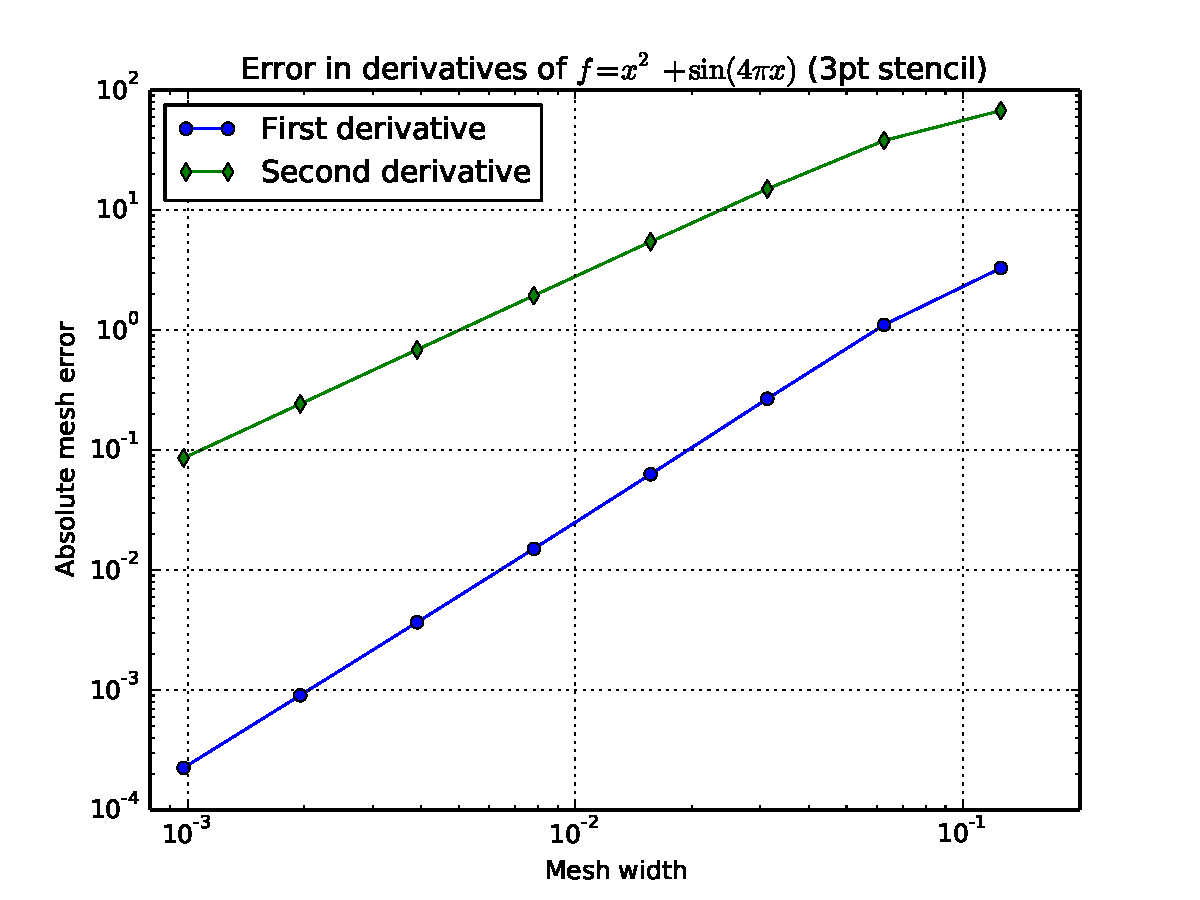
\includegraphics[width=\linewidth]{3PtStencilError.pdf}
\subsubsection*{ii.}
From the above graph, we can see that the first derivative error scales approximately with $h^2$ while the second derivative error scales with $h^{1.5}$. This is confirmed by finding the best polynomial fit using numpy.polyfit. According to the fitting, the first derivative scales as $h^{2.01}$ while the second derivative scales as $h^{1.41}$.

\subsubsection*{iii.}
In problem 1b), we estimated the error in the first and second derivatives at several different points. The relevant cases are the first case, which corresponds to the endpoints, and the third case, which corresponds to the interior points. From Eqns.\ 12 and 16, we predict the error at both the endpoints and then interior points of the first derivative to scale with $h^2$, which is exactly what we found from our program. 

For the second derivative, Eqn.\ 13 predicts an error of $h$ at the endpoints and Eqn.\ 18 predicts an error of $h^2$. While there are many more interior points than endpoints for small $h$, $h$ is also much larger than $h^2$ and thus each endpoint has a larger impact than an individual interior point. We would expect these effects to balance and yield a scaling somewhere between $h$ and $h^2$, which once again is what we see from our program.

\subsection*{b)}
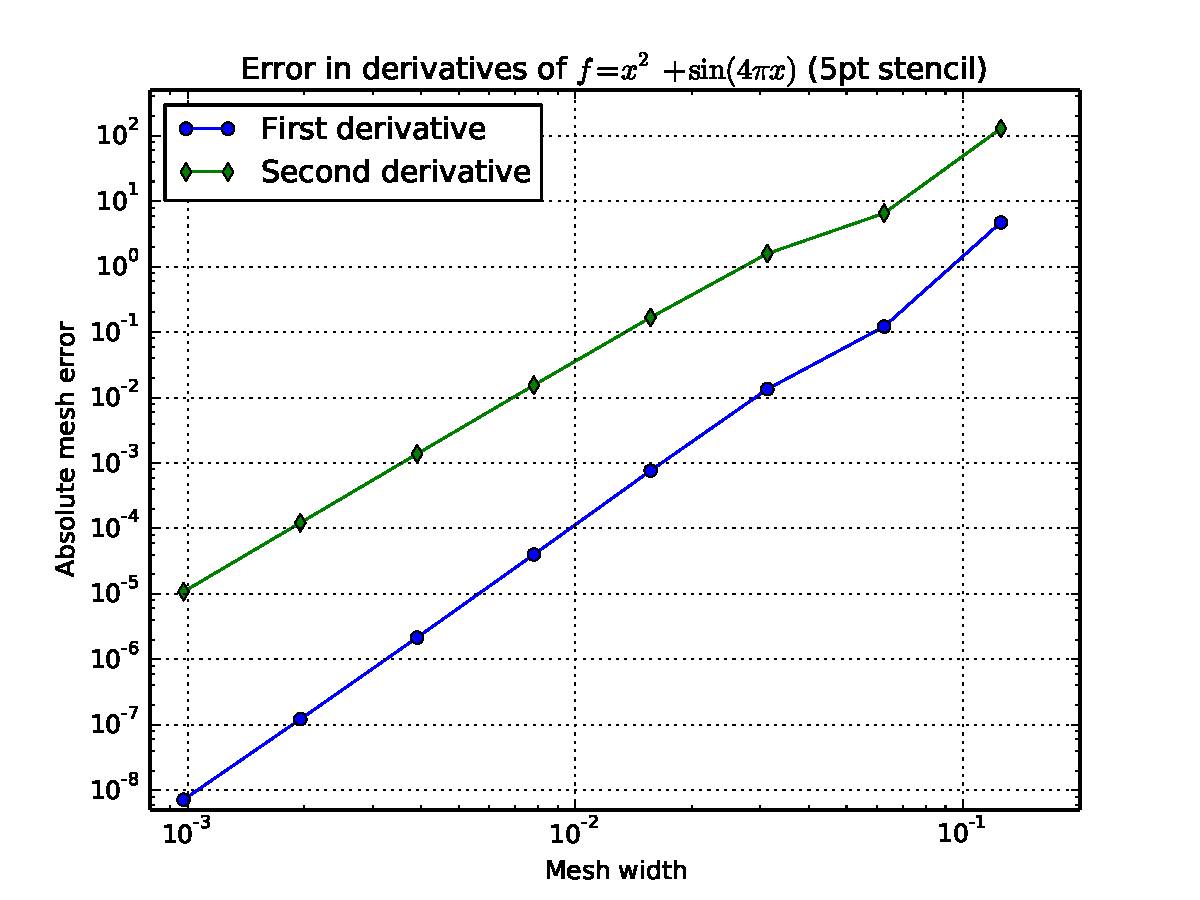
\includegraphics[width=\linewidth]{5PtStencilError.pdf}

From the above graph, we can see that the first derivative error scales approximately with $h^4$ while the second derivative error scales with $h^{3.5}$. This is confirmed by finding the best polynomial fit using numpy.polyfit. According to the fitting, the first derivative scales as $h^{4.13}$ while the second derivative scales as $h^{3.30}$.

The errors follow a similar trend to those in part a) but decreased by a factor of $h^2$ since we are using more points in our stencil calculation. The first derivative error is approximately an integer while the second derivative error is slightly higher than expected due to the difference between endpoints and interior points.

\section*{Problem 3}
\subsection*{a)}
\begin{equation}
-\frac{d^2u}{dx^2}=1\ \mathrm{for}\ x\in[0,1],\ u(0)=0,\ u(1)=1
\end{equation}

We can solve this problem by guessing a solution of the form:
\begin{equation}
u(x)=ax^2+bx+c
\end{equation}
and solving for appropriate $a$, $b$, and $c$.

First impose $u(0)=0$:
\begin{equation}
0+0+c=0\implies c=0
\end{equation}

Now impose $u(1)=1$:
\begin{equation}
a+b=1\implies b=1-a \implies u(x)=ax^2+(1-a)x
\end{equation}

Finally, impose $-\frac{d^2u}{dx^2}=1$:
\begin{equation}
-2a=1\implies a=-\frac{1}{2}
\end{equation}

So our solution is:
\begin{equation}
\boxed{u(x)=\frac{-x^2+3x}{2}}
\end{equation}

\subsection*{b)}
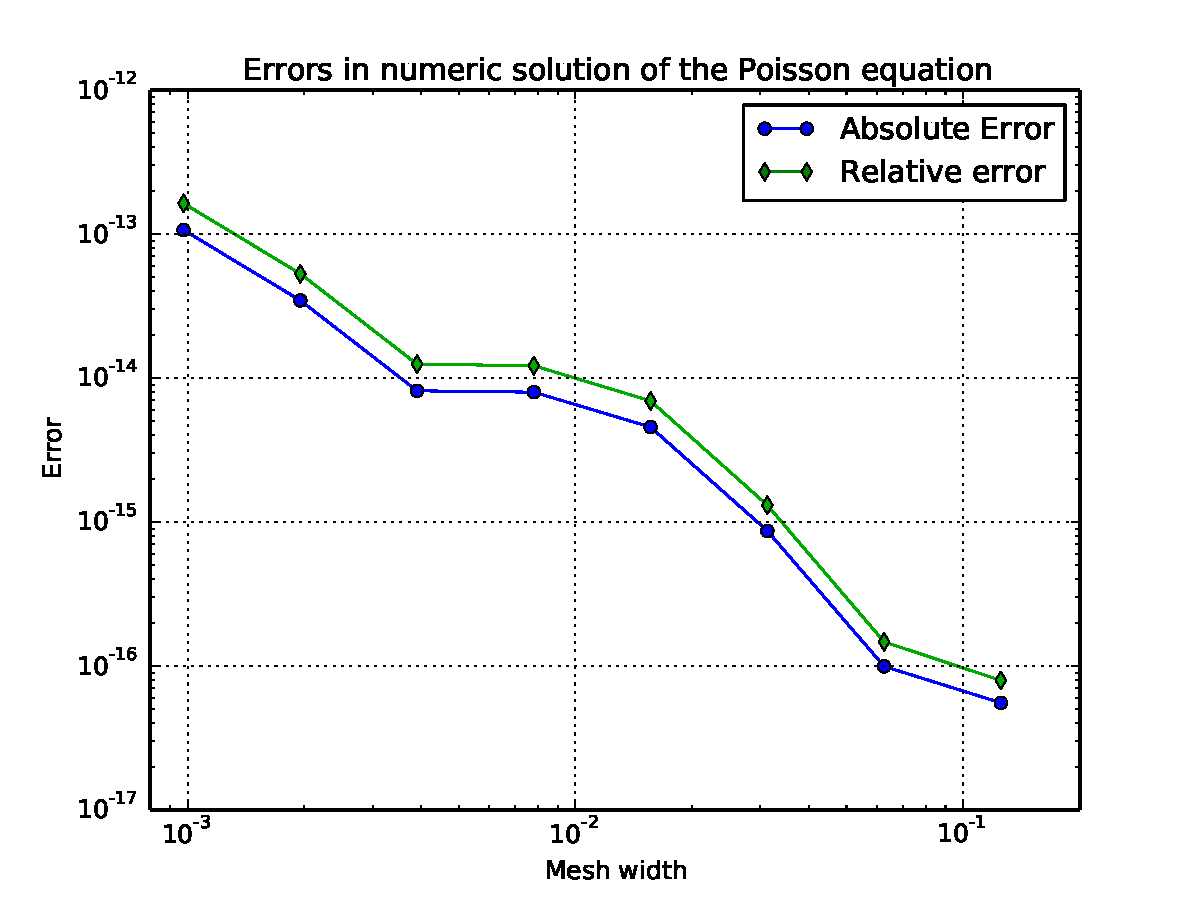
\includegraphics[width=\linewidth]{PoissonError.pdf}
\subsection*{c)}
From problem 1, we know the error in our first and second derivative calculations will come from third or higher order derivatives. However, our solution (Eqn.\ 24) has zero third and higher derivatives. The only errors in our program then must come from computer rounding errors which are generally of order $10^{-16}$. At each computation this error can be introduced. Since we impose boundary conditions, there is 0 error at the endpoints and the only error comes from the interior points. With a smaller mesh size, there are more interior points and more steps need to be done to reach the points that are further from the endpoints. These computer errors accumulate here causing the error to increase as the number of points increases.
\end{document}